In this chapter, we address the approach used for realizing IRS in kernel space. 
In the first section, we discuss a theoretical design. 
In the later sections, we address the potential challenges related to its implementation and the implementation of the prototypes.

\section{Theoretical Design \label{theor_des}}

Figure~\ref{design_overview} depicts the design overview of the IRS. 
Verifier and scheduler are the main components of IRS. 
Verifier is not an automated software.
However, there are some changes in the representation of some components such as the trace/scheduling constraints which are discussed in section \ref{vec_clk}.

\tikzstyle{custblock} = [rectangle, minimum width=3cm, minimum height=1cm, text centered, draw=black, fill=white!30]
\begin{figure}[h]
\centering
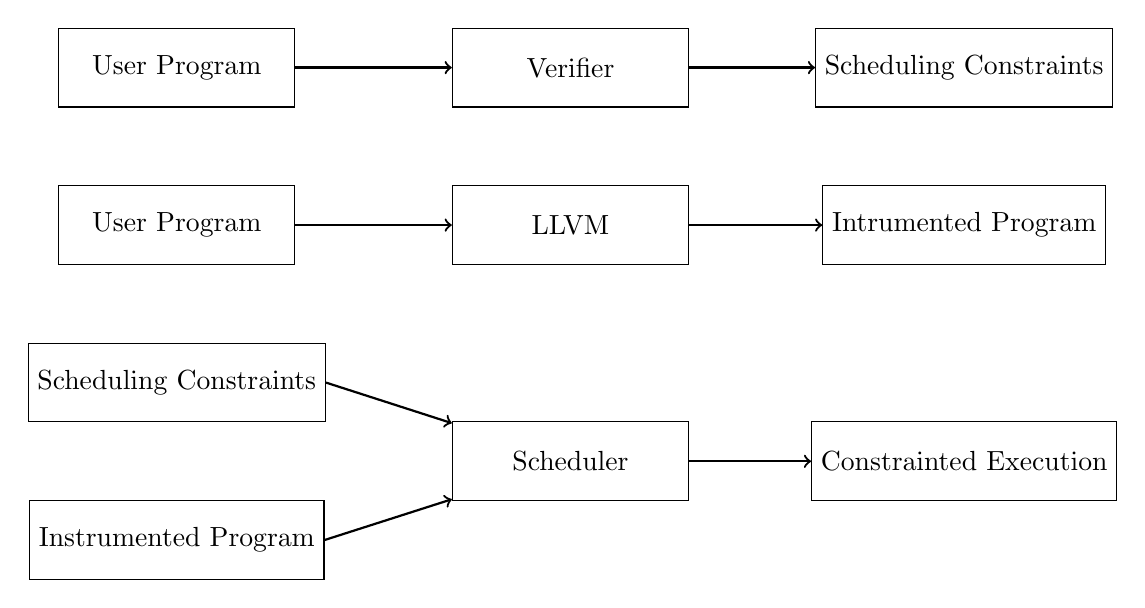
\begin{tikzpicture}[node distance=2cm]
%Custom blocks
\node (Us1) [custblock] {User Program};
\node (Us2) [custblock,below of=Us1] {User Program};
\node (ver) [custblock,right of=Us1,xshift =3cm] {Verifier};
\node (tr) [custblock,right of=ver,xshift =3cm] {Scheduling Constraints};
\node (llvm) [custblock,right of=Us2,xshift =3cm] {LLVM};
\node (ipgm) [custblock,right of=llvm,xshift =3cm] {Intrumented Program};
\node (Tr) [custblock,below of=Us2] {Scheduling Constraints};
\node (IPgm) [custblock,below of=Tr] {Instrumented Program};
\node (Sched) [custblock,right of=Tr,yshift=-1cm,xshift =3cm] {Scheduler};
\node (opgm) [custblock,right of=Sched,xshift =3cm] {Constrainted Execution};


%Arrows
\draw [->,thick] (Us1.east) -- (ver);
\draw [->,thick] (ver.east) -- (tr);
\draw [->,thick] (Us2.east) -- (llvm);
\draw [->,thick] (llvm.east) -- (ipgm);
\draw [->,thick] (Tr.east) -- (Sched);
\draw [->,thick] (IPgm.east) -- (Sched);
\draw [->,thick] (Sched.east) -- (opgm);
\end{tikzpicture}
\caption{IRS Design Overview}
\label{design_overview}
\end{figure}

The key component of this thesis is the scheduler. 
Scheduler handles the scheduling of various user level threads based on their memory access permissions. 
Memory access permissions are perceived by trace files. 
Trace files represent the execution order of shared memory events for the threads in a multithreaded program.  
The trace in a trace file is realized as simple graph with nodes. 
Each node denotes a shared memory event for a thread which can be a read or a write event. 
\\
\noindent\begin{minipage}{.45\textwidth}
\begin{lstlisting}[mathescape=true,style=customc,caption={Uninstrumented User Program},frame=tlrb,label={lst:uninstr_usr_pgm}]
Shared Variable: x;
Thread j($j \in 1..N$): 
......
x=0;	//shared memory access
....
\end{lstlisting}
\end{minipage}\hfill
\begin{minipage}{.45\textwidth}
\begin{lstlisting}[mathescape=true,style=customc,caption={Instrumented User Program},frame=tlrb,label={lst:instr_usr_pgm}]
Shared Variable: x;
Thread j($j \in 1..N$): 
......
BeforeMA();
x=0;	//shared memory access
AfterMA();
....
\end{lstlisting}
\end{minipage}

LLVM is another component part of the IRS framework. 
It primarily annotates the user program for shared memory events as shown in listing~\ref{lst:uninstr_usr_pgm} and \ref{lst:instr_usr_pgm}. 

%\subsection{Motivation \label{mot}}
%
%The scheduler implemented in the existing IRS framework addresses a user space implementation. 
%The user space adaptation of the scheduler focuses on two implementation variants. 
%The first user space implementation focuses on a busy waiting design and the second user space implementation uses a conditional variable setup. 
%Let us call the first implementation as IRS\_Sh and second one as IRS\_Opt for the sake of simplicity. 
%IRS\_Sh uses the pool of user threads created during the multithreaded program to block and signal other threads. 
%It uses the busy waiting design to block a certain thread and use other threads in the pool to signal from the wait. 
%IRS\_Opt uses an additional scheduler thread which takes care of requests for blocking or unblocking certain thread. 
%It uses condition variables to address the blocking or unblocking functionality of a given thread. 
%IRS\_Sh provides poor performance when the number of threads are more than the number of cores. 
%Busy waiting design performs poorly when the number of cores is less than the number of threads. 
%Whereas in case of IRS\_Opt, it uses conditional variables which is a synchronization abstraction provided by the pthread library. 
%In this thesis, we argue that such an implementation is expected to have high execution overhead when the amount of communication using the conditional variables increases. 
%The additional overhead in IRS\_Opt is expected to occur due to the library overheads from pthread library. 
%The term `amount of communication' is relative to the number of shared-memory events encountered in the multithreaded program. 
%
%Since both the user space solutions for the scheduler is expected to suffer from poor performance, we present a new approach of moving the scheduler logic to kernel space. 
%We expect to provide low execution overhead compared to the user space solutions. 
%In the rest of this chapter, we realize various ways to move the scheduler module to kernel space. 
%We expect to achieve good performance with the solutions presented in the rest of this chapter.

\subsection{Vector Clock \label{vec_clk}}

Vector clock is an algorithmic design motivated from Lamport logical clocks~\citep{fidge1991logical}. 
It is used to detect causality violations and generating a partial ordering of events in a distributed system. 
A vector clock is an array of N logical clocks corresponding to N processes/threads. 
Vector clocks allow for the partial causal ordering of events.
The following definition holds:
\begin{itemize}
\item $VC(x)$ denotes the vector clock of event $x$, and $VC(x)_a$ denotes the component of that clock for process $a$. 
\item $VC(x) < VC(y) \iff \forall a[VC(x)_a \lneq VC(y)_a] \wedge \exists b[VC(x)_b < VC(y)_b]$
\item $x \to y$ indicates event $x$ happened before event $y$. It is defined as : if $x \to y$, then $VC(x) < VC(y)$
\end{itemize}

The approaches discussed in this thesis uses a vector clock implementation for determining the number of memory events completed by a given thread, which is used to block or unblock a given thread. 
The trace file generated as graph representations are manually converted into strings of vector clock representations for using in this thesis. 
The vector clock representation only include the threads which are constrained. 
More details about the vector clock representation and traces can be found in the appendix~\ref{appendixc}.


\subsection{Design classes}

We have two different classes of approach used for this thesis. 
The two approaches can be classified as: design with proxy and design without proxy checking. 
Proxy checking referred above is the checking for memory  access permission for the thread based on the constraints set in the trace. 

\begin{lstlisting}[mathescape=true,style=customc,caption={Yield functionality and thread revival},frame=tlrb,label={lst:yield_func}]
Kernel Space:
yield(threadid j) {
	if(memory_access_permission(j)==restricted) {
		block_thread(j);
	}
}
reviveotherthreads() {
	for thread j($j \in 1..N$) except j is not the current thread:
		if(memory_access_permission(j)==allowed) {
			unblock_thread(j);
		}	
	}
}
\end{lstlisting}
From figure~\ref{design_overview}, it is evident that we require scheduling constraints/traces and the instrumented program for executing with the scheduler. 
The IRS implementation which this thesis is based upon, uses an LLVM implementation for instrumenting the user program. 
When instrumenting the user program, LLVM inserts function calls to two methods namely $BeforeMA()$ and $AfterMA()$ which are inserted in places before and after every shared memory access in the program as shown in Listing~\ref{lst:uninstr_usr_pgm} and \ref{lst:instr_usr_pgm}. 
The instrumented program is later, run with the scheduling constraints on the scheduler. 
The decision to block the thread is handled by the thread itself by invoking the yield functionality. 
A thread would block itself when it has no permission to access the shared memory. 
The decision making of the thread and the yield functionality are the only concepts discussed with the prototypes in this thesis. 

In this thesis, we propagate the decision making logic and yield functionality to kernel space as shown in Listing~\ref{lst:yield_func}. 
However, in case of the second approach used in this thesis we have an additional proxy checking for memory permissions in user space. 
We expect these propagations to yield a good performance compared to the user space solutions. 

\noindent\begin{minipage}{.45\textwidth}
\begin{lstlisting}[mathescape=true,style=customc,caption={First Approach},frame=tlrb,label={lst:first_approach}]
User Space:
Thread j($j \in 1..N$): 
//on activating a BeforeMA call
BeforeMA() {
	yield(j);
}
AfterMA() {
	reviveotherthreads();
}
\end{lstlisting}
\end{minipage}\hfill
\begin{minipage}{.45\textwidth}
\begin{lstlisting}[mathescape=true,style=customc,caption={Second Approach},frame=tlrb,label={lst:second_approach}]
User Space:
Thread j($j \in 1..N$): 
//on activating a BeforeMA call
BeforeMA() {
	if(memory_access_permission(j)==restricted) {
		yield(j);
	}
}
AfterMA() {
	reviveotherthreads();
}
\end{lstlisting}
\end{minipage}


\subsubsection{First Approach \label{fir_app}}

This approach has no proxy checking in the user space. 
When there is an occurrence of a shared memory event, this approach communicates to kernel space from the $BeforeMA()$ and $AfterMA()$ callback functions. 
These functions aid the logic of implementing yield functionality in the thread and also in reviving other threads. 
The pseudo code of this approach is depicted in listing~\ref{lst:first_approach}. 
Such an approach is suitable when the number of memory constraints are close to the total number of shared memory events in a multithreaded program. 
There are four design prototypes using this approach. 
Details related to these prototypes are discussed further in section \ref{nocheck}.

\subsubsection{Second Approach \label{sec_app}}

This approach has a proxy checking in the user space. 
When there is an occurrence of a shared memory event, this approach initially checks for memory access permission in user space and based on the outcome of the check, it communicates to the kernel space. 
$BeforeMA()$ and $AfterMA()$ functions are used in the same way as in first approach. 
However, with the only difference of having a proxy check for memory access permission inside the $BeforeMA()$. 
The pseudo code of this approach is depicted in listing~\ref{lst:second_approach}.
There are two design prototypes using this approach. More details about these prototypes are discussed further in section \ref{proxycheck}.
With the proxy checking in place, this design is expected to provide good performance when the following condition occurs: 

\begin{equation}
num\_memory\_constraints << total\_memory\_events
\label{mem_cond}
\end{equation}

$num\_memory\_constraints$ represents the number of memory constraints provided in the trace file for the multithreaded program and $total\_memory\_events$ indicates the total number of shared memory events present in the same multithreaded program.
This approach reduces the number of unnecessary yield calls made to kernel space, which reduces drastic overhead generated by communication and waiting in kernel space. 
When the above condition fails, this approach would behave like the first approach, but would have higher overhead because of the proxy checking in user space. 
Under such scenarios, the prototypes under the first approach is expected to provide a good performance. 


\section*{Note}
In the progression of this document, we would be using certain acronyms to indicate certain meanings. 
Some of them are:
\begin{itemize}
\item \textbf{UTID} - User defined thread ID which is relative inside the user program. 
\item \textbf{RTID} - Real Thread ID which is assigned within the proc file system for any thread created within the user land. 
\item \textbf{TaskID} - All threads are internally realized as tasks in kernel space and are allocated with an identifier which is task ID.
\item \textbf{API} -Application Programming Interface.
\end{itemize}

\section{Design Challenges}

In this section, we address some of the challenges we might face when moving the scheduling decisions of IRS to kernel space.

\subsection{Mapping UTID to Task Object}

UTID  is passed to kernel space via a custom proc file and invoking scheduler API - $get\_current\_task()$. 
This function returns a task struct object. 
In kernel space, we can have a mapping of UTID to the obtained task struct object. 
User defined thread ID (UTID) is required to be communicated to the scheduler. 
And the mapping of task struct to UTID needs to be realized, in order for the scheduling to be done right. 
The custom registration proc file communicates the UTID to the kernel space. 
The user defined thread writes the UTID in the above proc file, which would trigger a callback to the write function in the kernel space module. 
Threads will be created based on the user's choice. 
On thread creation, the threads would invoke the registration module individually. 
This method would require a definition of synchronization block inside the kernel space since, multiple write function calls are invoked. 
Multiple threads are accessing the registration module. 
The synchronization is also required between the scheduler module and registration module.


\subsection{Data Structure for mapping UTID to Task Object}

The mapping of UTID - task object is realized, when the registration of a UTID to the scheduler is done. 
In the registration, the user thread is required to pass the UTID. 
The task object is obtained by invoking $get\_current\_task()$ function during registration call. 
A data structure is created to store the mapping of UTID to task object. 
An item in the data structure is created whenever a registration of UTID takes place. 
An item is otherwise accessed during the invocation of $context\_switch()$ function. 
In a user space environment, there are solutions such as dictionary mapper or even hash table designs. 
Since the mapping is coherent in the kernel space, possible design choices include - linked list, arrays. 
There is a complexity associated in accessing a node in the linked list, which is O(n).

\subsection{Communication between user thread and kernel space scheduler during context switch} 

With the transition of scheduler to kernel space, there is a need of having a communication design to interact between the user program and kernel space scheduler. 
The communication can be dealt in many ways\cite{commkernelanduser}. 
Some of them are:

\begin{itemize}
\item ProcFS - Virtual file system for handling process and thread information base. Useful for small and short communications. 
\item Netlink - Special IPC scheme between kernel space and user space which uses sockets. However, extremely expensive when opening and closing of sockets.
\item System call - Functional implementation mainly meant to communicate some data or perform a specific service in kernel space. It requires a static implementation in the kernel source tree. Extremely hard to develop and debug the implementation.
\item CharacterDevice - Special buffering interface provided for communicating with character device driver setups.
\item Mmap - Fastest way of copying data between kernel space and user space without explicit copying. Useful for large transactions of data.
\item Signals - Unidirectional communication. Communicated from kernel space to user space. 
\item Upcall - Execute a certain function defined in the user space from kernel space.
\item IOCTL - Used primarily for input and output operations in between user space and kernel space. It is an extension of character device implementation. It uses simple read and write system calls for communication purposes. It can be realized as an alternative for system call.

\end{itemize}


Assessing the requirements for the implementation, IOCTL seems to be a perfect fit for all the interactions required for a scheduler module. 
System call implementation requires the building of the entire kernel source tree and they are very difficult to debug and develop. 
IOCTL provides the possibility for a plug and play design.

\subsection{Mapping the trace object to kernel space}

The proposed design uses vector clocks as an outline for trace implementation. 
The traces generated as graphs are mapped to kernel space as a struct object. 
Graphs are realized as graphviz files. 
Parsing of graph is required before they are mapped to the kernel space. 
The parsed graph is passed to the kernel space as a long string via a custom proc file. 
Currently, there is no automated method existent in this thesis to generate a graph string from a graphviz file. 
We generate the trace string manually and pass it as an input to the custom proc file when the user program starts.

\subsection{Trace verification inside user program vs kernel space scheduler}

On occurrence of a shared memory event, the respective callbacks (BeforeMA() \& AfterMA() - Before memory access and After memory access) from the user program would trigger an IOCTL call to the kernel module. 
Such a design would facilitate towards a non-preemptive scheduler. 
By overcoming the additional synchronization overhead existent in the user space design, we encounter the problem of invoking IOCTL calls  for accessing the kernel module. 
In a monolithic kernel architecture, most of the IOCTL calls are blocking synchronous calls to the kernel space. 
Having too many IOCTL calls would increase the scheduler overhead on the program execution. 
One solution is to make IOCTL calls when there is an actual need of a  context switch~\citep{flexsc}. 
The user space threads would assess the trace based on which the IOCTL calls for the kernel space scheduler would be made. 
We discuss about such a solution in two prototypes used in the implementation section.

Note - Non-preemptiveness indicated in this section and the rest of the document is in regard to the scheduler implemented in this thesis and not the OS Scheduler.

\subsection{Yield to scheduler vs Preemptive scheduler}

The current implementation uses a non-preemptive design for the scheduler. 
The design uses the verification of memory access event and performs yield to scheduler when the access to memory is not permitted. 
A preemptive design would reduce the communication between user space and kernel space during context switch but, would increase the same for every memory access events. 
With such an implementation, it would require the kernel space to be able to detect the memory access events of the global memory used by the user space threads. 
Considering the complexity of its implementation and lack of existing solutions such a design would be not feasible to implement. 


\subsection{Vector clock design for finding the event in the trace}

Before a shared memory access is made, the user thread triggers a callback - \emph{BeforeMA()} (in short before memory access). 
The callback internally triggers a yield to scheduler if the memory access is not permitted. 
The memory access permission is determined by checking the trace object. 
The timeline of the event is required to be addressed during the checking with the trace. 
The event timeline can be determined by having a vector clock design. 
The same vector design needs to be used inside the kernel space as well, for its trace verification function.


%----Implementation section------%

\section{Synchronization Designs \label{sync_des}}

As discussed in the previous sections, we classify the designs into two classes. 
The classification is based on the checking for memory permission in user space. 
The first class has no checking for memory permission in the user space and the second has a proxy checking in user space for memory permission. 
Tables~\ref{protos_without_proxy} and \ref{protos_with_proxy} depict this classification.

\begin{table}[h]
\begin{center}
 \begin{tabular}{|c c c|} 
 \hline
 & Shared Thread & Separate Thread\\ %[0.5ex] 
 \hline
Semaphore & Prototype 1 & Prototype 2\\
Scheduler APIs & Prototype 3 & Prototype 4\\
\hline
\end{tabular}
\end{center}
\caption{Prototypes without proxy checking}
\label{protos_without_proxy}
\end{table}

\begin{table}[h]
\begin{center}
 \begin{tabular}{|c c c|} 
 \hline
 & Shared Thread & Separate Thread\\ %[0.5ex] 
 \hline
Semaphore &  & Prototype 5\\
Scheduler APIs &  & Prototype 6\\
\hline
\end{tabular}
\end{center}
\caption{Prototypes with proxy checking}
\label{protos_with_proxy}
\end{table}

The yield functionality depicted in all the prototypes either use a semaphore based solution or scheduler APIs. To get a better understanding about semaphores and scheduler APIs please refer to appendix C.

The implementation of all prototypes comprise of three loadable kernel modules: thread registration, trace control and scheduler. 
The scheduler module is the only module implemented differently for all the prototypes.

\subsection{Trace Registration}

\begin{figure}[h]
\centering
\begin{tikzpicture}[scale=0.9,transform shape]
 
  % Draw diagram elements
  % trace registration area
  \path \spacelayer {TRACEFILE}{Trace File}{};  
  \path (TRACEFILE.south)+(0.0,-2.0)\spacelayer {TRACEOBJ}{Trace Object}{};  
  \path (TRACEOBJ.east)+(5.0,0.0) \spacelayer {TRACEPROCFS}{Trace Reg File}{};
  \path (TRACEPROCFS.east)+(4.5,0.0) \spacelayer {TRACESYSCALL}{Syscall\\ trace}{};  
  \path (TRACESYSCALL.south)+(0.0,-3.0) \spacelayer {TRACECALLBACK}{Trace Write Callback}{};
  
  % Draw arrows between elements

  %thread registration block
  \path [line] (TRACEFILE.south) -- node [left] {$trace$}
									 node [right] {$file$} (TRACEOBJ);
  \path [line] (TRACEOBJ.east) -- node [above] {$trace\_reg()$} (TRACEPROCFS);

  \path [line] (TRACEPROCFS.east) -- node [above] {$write()$} (TRACESYSCALL);
  
  \path [linepart] (TRACESYSCALL.south) -- node [left] {$callback$}
                                 node [right]{$triggered$} (TRACECALLBACK);  
  
  %background generation block
  \background{TRACEFILE}{TRACEFILE}{TRACEOBJ}{TRACEOBJ}{User Space}
  \background{TRACESYSCALL}{TRACESYSCALL}{TRACECALLBACK}{TRACECALLBACK}{Kernel Space}

\end{tikzpicture}
\caption{Trace Registration}
\label{trace_reg}
\end{figure}
The trace file is passed on as an input for the scheduler. 
In figure~\ref{trace_reg}, the trace file is read by the main user thread at the start of its execution. 
It parses the file, creates and passes the trace object to the kernel space as string via a custom file created in the proc file system. 
Trace registration is implemented within the trace control module. 
The trace control module deals with the manipulation of trace object in the kernel space. 
Trace control module is imported into the scheduler module for obtaining the trace control functionality and also to access the trace itself. 
\subsection{Thread Registration}

\begin{figure}[h]
\centering
\begin{tikzpicture}[scale=0.9,transform shape] 
  
  % thread registration block area
  \path \spacelayer {THREADINIT}{Thread\\ Created}{};  
  \path (THREADINIT.south)+(0.0,-2.0)\spacelayer {USERTHREADREG}{Thread\\ Registration}{};  
  \path (USERTHREADREG.east)+(5.0,0.0) \spacelayer {REGPROCFS}{Registration File}{};
  \path (REGPROCFS.east)+(4.5,0.0) \spacelayer {REGSYSCALL}{Syscall\\ Thread\\ Registration}{};
  \path (REGSYSCALL.south)+(0.0,-2.0) \spacelayer {REGCALLBACK}{Write Callback}{};

  \background{THREADINIT}{THREADINIT}{USERTHREADREG}{USERTHREADREG}{User Space}
  \background{REGSYSCALL}{REGSYSCALL}{REGCALLBACK}{REGCALLBACK}{Kernel Space}
  
   %Draw arrows between elements
   %thread registration block
  \path [line] (THREADINIT.south) -- node [left] {$register$}
									 node [right] {$thread$} (USERTHREADREG);
  \path [line] (USERTHREADREG.east) -- node [above] {$reg\_thread()$} (REGPROCFS);

  \path [line] (REGPROCFS.east) -- node [above] {$write()$} (REGSYSCALL);
  
  \path [linepart] (REGSYSCALL.south) -- node [left] {$callback$}
                                 node [right]{$triggered$} (REGCALLBACK);

\end{tikzpicture}
\caption{Thread Registration}
\label{thread_reg}
\end{figure}
In figure~\ref{thread_reg}, the registration block happens when a user thread is created. 
The registration happens via a custom proc file system. 
For convenience a $thread\_reg()$ method is invoked in the user space, which internally registers the thread to the kernel space. 
The thread registration implementation is done entirely in thread registration kernel module. 
This registration is used to allocate memory space for bookkeeping the thread entry in scheduler. 
%\newpage
\begin{lstlisting}[mathescape=true,style=customc,caption={Pseudo Code for checking memory access permission},frame=tlrb,label={lst:check_perm}]
mem_access = {allowed, restricted};
check_mem_acc_perm(curr_vec_clk, traceobj, thread_id tid) {
	if(clock[tid] is same in traceobj and curr_vec_clk) {
		$\forall$thread_id i in {{1...N}-{tid}}:
		if clock[i] in traceobj is greater to the one in curr_vec_clk) {
			return restricted;		
		}	
	}
	else if(clock[tid] in traceobj is lower than one curr_vec_clk) {
		return restricted;	
	}
	return allowed;
}
\end{lstlisting}


\subsection{IOCTL Manager}

\begin{figure}[h]
\centering
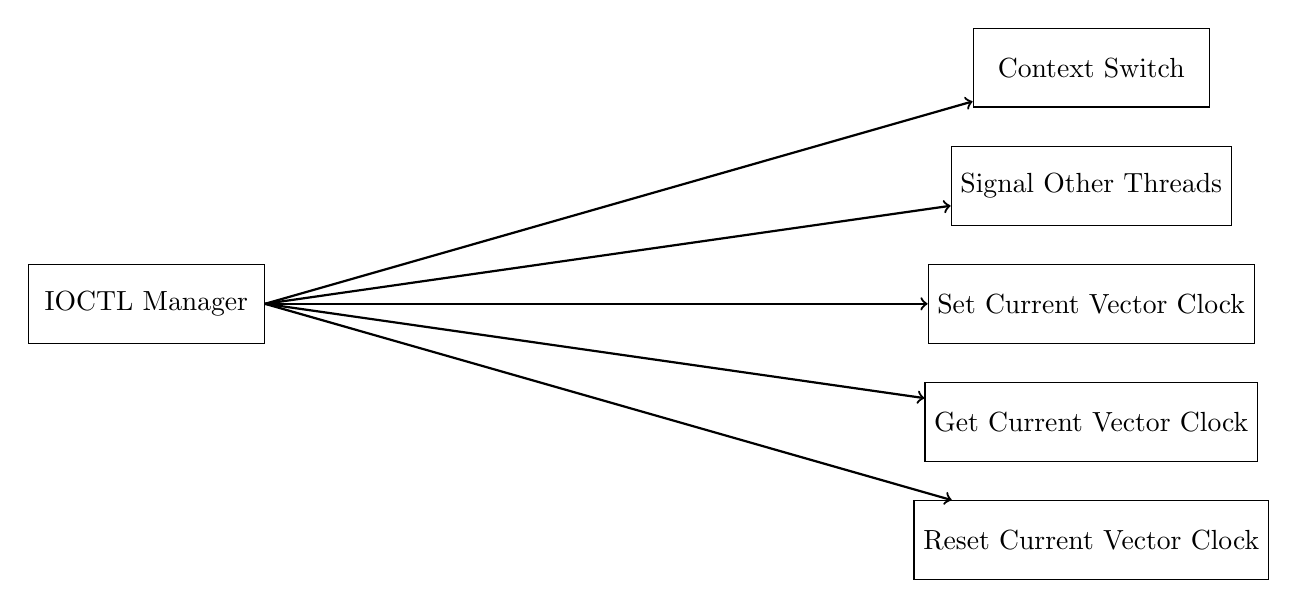
\begin{tikzpicture}[scale=0.7, node distance=2cm]
%Custom blocks
\node (ioctlmgr) [custblock] {IOCTL Manager};
\node (ctxtswitch) [custblock,right of=ioctlmgr,xshift =10cm,yshift =3cm] {Context Switch};
\node (signalothers) [custblock,right of=ioctlmgr,xshift =10cm,yshift =1.5cm] {Signal Other Threads};
\node (setclk) [custblock,right of=ioctlmgr,xshift =10cm] {Set Current Vector Clock};
\node (getclk) [custblock,right of=ioctlmgr,xshift =10cm,yshift =-1.5cm] {Get Current Vector Clock};
\node (resetclk) [custblock,right of=ioctlmgr,xshift =10cm,yshift =-3cm] {Reset Current Vector Clock};


%Arrows
\draw [->,thick] (ioctlmgr.east) -- (ctxtswitch);
\draw [->,thick] (ioctlmgr.east) -- (signalothers);
\draw [->,thick] (ioctlmgr.east) -- (setclk);
\draw [->,thick] (ioctlmgr.east) -- (getclk);
\draw [->,thick] (ioctlmgr.east) -- (resetclk);
\end{tikzpicture}
\caption{IOCTL Manager}
\label{ioctl_mgr}
\end{figure}
IOCTL Manager is an abstraction layer in the kernel space used to contain any commands triggered from the user space. 
The manager acts as an interface for the commands requested by user space for kernel level services. 
It provides five different commands of operation as shown in figure~\ref{ioctl_mgr}. 
Among the five operations, three operations deal with the vector clock manipulation. 
The commands $context\_switch$ and $signal\_other\_threads$ are generally very expensive commands when invoked. 
You can observe their implementation in later sections of this chapter. 
$context\_switch$ command is used by all prototypes when there is a need to yield to the scheduler. 
$signal\_other\_threads$ command is used by  prototypes 1 and 3, the threads signal among themselves. 
In case of prototypes other than 1 and 3, $set\_clk$ command is used more frequent for updating a given thread's memory event. 
Updating the vector clock is a short operation when compared to signaling other threads. 
The prototypes 1 and 3 are expected showcase poor performance when encountered with the condition: $num\_memory\_constraints << total\_memory\_events$. 
These prototypes invoke $signal\_other\_threads$ command for every shared memory event thus, having a poor performance. 
Reset vector clock is invoked at the completion of the user program for resetting the clock and using it for the next execution. 
Get current vector clock is used to obtain the entire vector clock during the time of invocation. 
This command is primarily used for debugging purposes. 


\subsection{Design with no checking in user space \label{nocheck}}

In the following designs, we address the use of check for memory access  permission method entirely in kernel space. 
The pseudo code for the checking for memory access permission is depicted in listing~\ref{lst:check_perm}. 
All the prototypes in this thesis would be using the implementation shown in listing~\ref{lst:check_perm} for checking the memory access permission.

\subsubsection{Design with no additional scheduler thread} \label{no_check_no_add}

The design described in this section addresses the use of no additional scheduler thread. 
Prior to any global memory access, the given design would invoke IOCTL command with $context\_switch$ and thread id of the thread which addressed the memory event as its parameters. 
Prototypes 1 and 3 primarily works with a similar implementation. 
These prototypes defer in place of blocking and unblocking of the threads. 
Listing~\ref{lst:proto1} depicts the pseudo code of prototype 1.
\newpage
\begin{lstlisting}[mathescape=true,caption={Pseudo Code for Prototype 1}, style=customc,frame=tlrb,label={lst:proto1}]
User Space:
Thread j($j \in 1..N$):
BeforeMA() {	
	ioctl(CONTEXT_SWITCH, thread_id);	
}

AfterMA() {	
	ioctl(SIGNAL_OTHER_THREADS, thread_id);
}

Kernel Space:
semaphore threads_sem[1..N] = {0...0};
Queue waitqueue={}
ctxt_switch_thread(thread_id tid) {	
	if(check_perm(tid)==restricted) {
		signal_all_other_threads(tid);
		waitqueue.push(tid);
		down(threads_sem[tid]); 
	}
}
signal_all_other_threads(thread_id tid) {
	$\forall$ thread_id i in {{1...N}-{tid}}:
		if(i in waitqueue and check_perm(i)==allowed) {
			waitqueue.remove(i);
			up(threads_sem[i]);
		}
}

\end{lstlisting}

\subsubsection{Design with an additional scheduler thread}\label{sec_add_thread}

In this design, we have an additional scheduler thread which addresses the signaling mechanism pertained in the previous design. 
By having an additional scheduler thread, we move the entire signaling system to the scheduler thread.
Thus, reducing the execution overhead encountered in the pool of user space threads for signaling other threads.
The major changes are in kernel space code. 
However, there are minor variations in the $AfterMA()$ in user space. 
Inside the $AfterMA()$ call, we invoke the $set\_clk$ command. 
It is used to update the memory event for the thread which encountered the memory event. 
Prototypes 2 and 4 follow similar implementation. 
However, they defer in the blocking and unblocking mechanism of the thread. 
\newpage
\begin{lstlisting}[mathescape=true,caption={Pseudo Code for Prototype 2}, style=customc,frame=tlrb,label={lst:proto2}]
User Space:
Thread j($j \in 1..N$):
BeforeMA() {	
	ioctl(CONTEXT_SWITCH, thread_id);	
}

AfterMA() {	
	ioctl(SET_CLK, thread_id);
}

Kernel Space:
semaphore threads_sem[1..N] = {0...0};
Queue waitqueue={};

Run a kernel level thread every 1ms which invokes signal_permitted_threads function.

ctxt_switch_thread(thread_id tid) {	
	if(check_perm(tid)==restricted) {
		waitqueue.push(tid);
		down(threads_sem[tid]); 
	}
}
set_clk(thread_id tid) {
	vec_clk[tid]++;
}
signal_permitted_threads() {
	$\forall$ thread_id i in {1...N}:
		if(i in waitqueue and check_perm(i)==allowed) {
			waitqueue.remove(i);
			up(threads_sem[i]);
		}
}
\end{lstlisting}

\subsection{Design with proxy checking in user space\label{proxycheck}}

In the following designs, we address the use of checking for memory access permission both in user space and kernel space.

\subsubsection{Design with no additional scheduler thread}

Without an additional thread in kernel space, the design would require a signaling function inside $AfterMA()$, similar to the one used in Design~\ref{no_check_no_add} with no additional scheduler thread. 
Triggering a signaling mechanism is an additional overhead on the thread calling the $AfterMA()$. 
Therefore, such a design is not a wise choice when considering the performance metrics such as execution time.
 
\subsubsection{Design with an additional scheduler thread}

The scheduler implementation is similar to one defined in the section \ref{sec_add_thread} with an additional scheduler thread. 
Key difference is the additional checking for memory access permissions in the user space. 
The major changes are in user space code. 
Prototypes 5 and 6 use a similar setup as shown in listing~\ref{lst:proto5}. 
However, they differ in their blocking and unblocking mechanism of threads. 
As explained in the previous sections, this design is expected to perform better if the condition indicated in  equation~\ref{mem_cond}.
\begin{lstlisting}[mathescape=true,caption={Pseudo Code for Prototype 5 and 6}, style=customc,frame=tlrb,label={lst:proto5}]
User Space:
Thread j($j \in 1..N$):
BeforeMA() {	
	if(check_perm(j)==restricted) {
		ioctl(CONTEXT_SWITCH, thread_id);	
	}
}

AfterMA() {	
	ioctl(SET_CLK, thread_id);
}
//Rest of the code remains the same.
\end{lstlisting}
\subsection{Variant in blocking implementation}

In the previous designs, the blocking was done using semaphores. 
In the variant design, we use the combination of $schedule()$ and $wake\_up\_process()$ functions provided by the Linux scheduler APIs. 
The kernel level tasks associated for the provided user level threads are moved from running queue to wait queue by initially setting the task status as $TASK\_INTERRUPTIBLE$ and yielding the processor by invoking $schedule()$. 
The task added in wait queue is later resumed, when $wake\_up\_process(sleeping\_task)$ is invoked by another task(primarily another thread). 
On calling the $wake\_up\_process(sleeping\_task)$, the task status for $sleeping\_task$ is set as $TASK\_RUNNING$. 
It would be pushed to run queue and executed in future by the operating system scheduler on the basis of scheduler class and priority of tasks in run queue. 
Prototype 3,4 and 6 utilizes this design.
Listing~\ref{lst:proto3} and \ref{lst:proto4} depicts Prototypes 3 and 4.  
\newpage
\begin{lstlisting}[mathescape=true,caption={Pseudo Code for Prototype 3}, style=customc,frame=tlrb,label={lst:proto3}]
//rest remains the same.
Kernel Space:
Queue waitqueue={}
ctxt_switch_thread(thread_id tid) {	
	if(check_perm(tid)==restricted) {
		signal_all_other_threads(tid);
		waitqueue.push(tid);
		set_current_task_state(TASK_WAIT);
		schedule();
	}
}
signal_all_other_threads(thread_id tid) {
	$\forall$ thread_id i in {{1...N}-{tid}}:
		if(i in waitqueue and check_perm(i)==allowed) {
			waitqueue.remove(i);
			wakeup_process(taskforthreadid(i));
		}
}
\end{lstlisting} 
\begin{lstlisting}[mathescape=true,caption={Pseudo Code for Prototype 4}, style=customc,frame=tlrb,label={lst:proto4}]
//rest remains the same.
Kernel Space:
Run a kernel level thread every 1ms which invokes signal_permitted_threads function.
Queue waitqueue={}
ctxt_switch_thread(thread_id tid) {	
	if(check_perm(tid)==restricted) {	
		waitqueue.push(tid);
		set_current_task_state(TASK_WAIT);
		schedule();
	}
}
signal_permitted_threads() {
	$\forall$ thread_id j in {1...N}:
		if(j in waitqueue and check_perm(j)==allowed) {
			waitqueue.remove(j);
			wakeup_process(taskforthreadid(j));
		}
}
//rest remains the same.
\end{lstlisting}

\subsection*{Additional Note}

We have $signal\_all\_other\_threads()$ method invoked within $ctxt\_switch\_thread()$ method in Prototypes 1 and 3. 
The above call is made from $ctxt\_switch\_thread()$ to ensure that the design does not run into any deadlocks. 

A $waitqueue$ is used in all the prototypes. 
It is used to maintain a bookkeeping for all the blocked threads. 
A design without $waitqueue$ would require the checking memory access permission with the trace to be done differently. 
The modified design would have all the signaling threads checking the trace for all threads which could be blocked and signaling all the blocked threads independently whereas, in the design discussed in this thesis we use a $waitqueue$. 
The waitqueue is implemented as an array of boolean values and with size of total number of threads. 
To check if a thread is blocked or not, we can access array with the thread's id as its index. 
Firstly, such a modified design highlights a possibility of a race conditions when removing a memory event from a trace. 
A memory event is removed from the trace once the event is completed. 
Secondly, the prototypes using semaphores(Prototypes 1,2 and 5) could not be adapted with such design changes. 
Let us consider that, there are 4 threads in the multithreaded program. 
Three of the threads are running, whereas the last thread is blocked. 
When all first three threads invoke the $signal\_other\_threads()$ method, they would perform the $up$ operation on the semaphore variable meant for last thread(assuming that the fourth thread is allowed to execute). 
Problem here is that the value of the semaphore say $sema_4$ would be 3 and not one, value 3 would indicate the fourth thread to miss the yield functionality for the next three restricted memory access. 
As indicated in the appendix~\ref{appendixc}, we use a binary semaphore and not a counting semaphore for the threads in Prototypes 1,2 and 5. 
To avoid the race conditions, we could have a mutex around the code section which deals with the removal of the memory event from the trace. 
Invoking mutexes or locks regularly can affect the performance of the multithreaded program~\citep{torrellas1994false}. 
Having a mutex inside this code section would increase the execution overhead drastically. 
Moreover, such a design with mutex would make the design  to be logically equivalent to the one with the $waitqueue$. 
Therefore, there is no gain in making such a change. 

The algorithmic time complexity for running $signal\_all\_other\_threads()$ is $O(n^2)$, whereas $set\_clk()$ is $O(1)$. 
In $ctxt\_switch\_thread()$ method we have higher algorithmic time complexity in Prototypes 1 and 3, since they invoke $signal\_all\_other\_threads()$ internally.